\documentclass[10pt]{article}

\usepackage[cp1251]{inputenc}
\usepackage[T2A]{fontenc}
\usepackage[russian, english]{babel}

\usepackage{amssymb, amsmath, textcomp, tabularx, graphicx}

\newcolumntype{C}{>{\centering\arraybackslash}X}

\let \eps \varepsilon

\title{Задание 5}
\author{Коновалов Андрей, 074}
\date{}

\begin{document}

\maketitle

\noindent
\begin{tabularx}{\textwidth}{|C|C|C|C|C|C|C|C|C|C|}
  \hline
  1 & 2 & 3 & 4 & 5 & 6 & 7 & 8 & 9 & $\Sigma$ \\
  \hline
  &&&&&&&&& \\
  \hline
\end{tabularx}

\bigskip

{\bf Задача 1}

Результат поиска в глубину представлен на на рисунке. Дипы дуг графа указан около дуг, а значения функций $d$ и $f$ в скобках после названия вершины.

\centerline{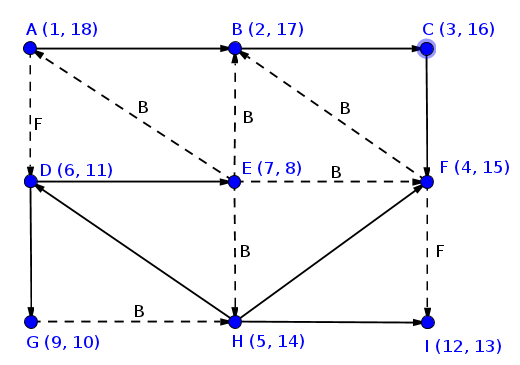
\includegraphics{1.png}}

\medskip

{\bf Задача 2}

{\it (i)}
Критерий не верный, контрпример:

\centerline{\includegraphics{{2.1}.png}}

{\it (ii)}
Критерий не верный, контрпример:

\centerline{\includegraphics{{2.2}.png}}

\medskip

{\bf Задача 4}

{\it (i)}
Критерий не верный, контрпример:

\centerline{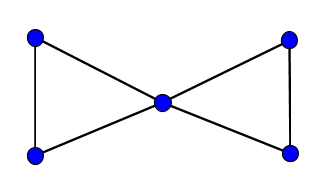
\includegraphics{4.png}}

\medskip

{\bf Задача 5}

{\it (i)}
Точки раздела: $\{ D, H, I, L \}$.
Мосты: $\{ GH, HI \}$.
Двусвязные компоненты: $\{ ABNO, DELM, LKFIJ \}$

\end{document}
